\documentclass[a4paper]{article}

\usepackage[pdftex]{graphicx}
\usepackage{xspace}

\def\G#1{\texttt{G#1}\xspace}
\def\P#1{\texttt{P#1}\xspace}
\def\D#1{\texttt{D#1}\xspace}

\parindent 0pt
\parskip 0pt

\begin{document}

\title{How Pulley Produces Incremental Output}
\author{Rick van Rein}
\maketitle
\begin{abstract}\noindent\em
The Pulley script langauge provides a manner of specifying, almost in a SQL style, how variables from various places in LDAP should be related to produce output.  The implementation is incremental, making Pulley a very pragmatic component to pass through changes rather than complete new configurations.  But how is this done?
\end{abstract}

First, during analysis of the Pulley script, the variabels mentioned in each line is noted.  Conditions can only be computed when all their variables are known, and this results in a partitioning of variables.  For each partition, there is a set of conditions that can be computed over them.  Variables that are not subjected to conditions form partitions of their own.


\section{Deriving impacted drivers}

Generators produce tuples containing variables, and drivers output variables.  This leads to a notion of overlap between these entities.  The figure below uses \G{$i$}, \P{$j$} and \D{$k$} to encode generator $i$, variable partition $j$ and driver $k$, respectively.

\centerline{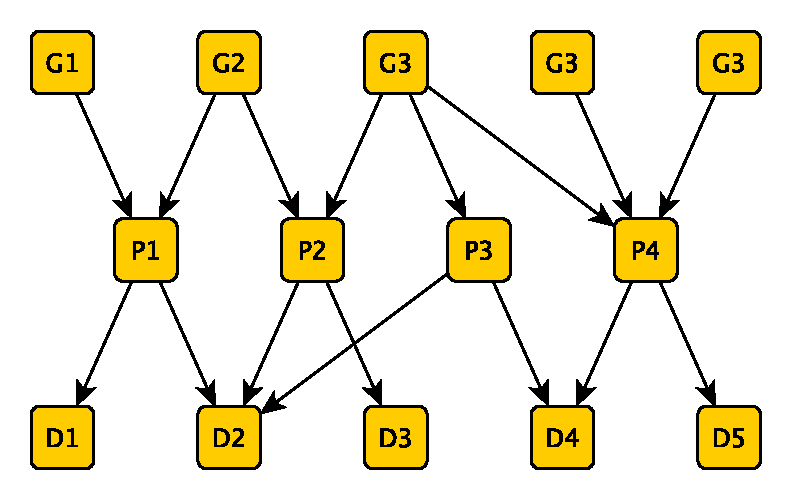
\includegraphics[scale=0.5]{img/network0-varoverlap.pdf}}

Now let's assume that an update arrives on generator \G2 forks a tuple addition (or removal, which is similar except for its impact on the driver).  We use the red colour to indicate downward reasoning and draw:

\centerline{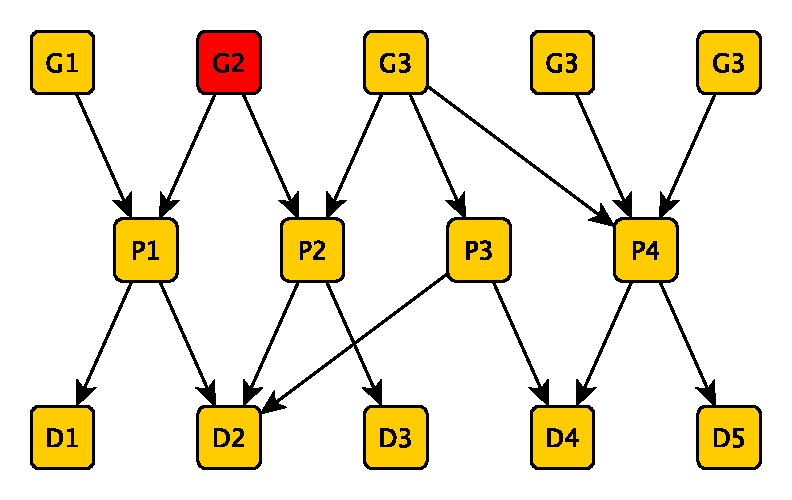
\includegraphics[scale=0.5]{img/network1-generate.pdf}}

This generator produces variables that are constrained by conditions, represented by variable partitions \P1 and \P2,

\centerline{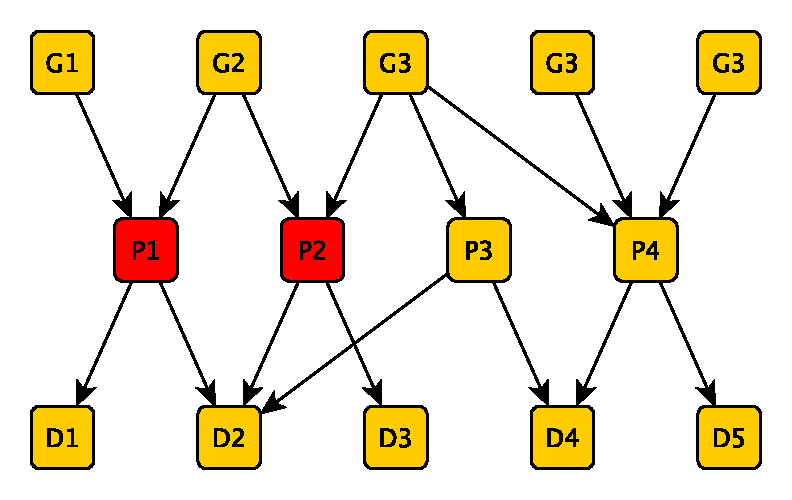
\includegraphics[scale=0.5]{img/network2-varparts.pdf}}

These partitions may impact a number of drivers, in this case \D1, \D2 and \D3:

\centerline{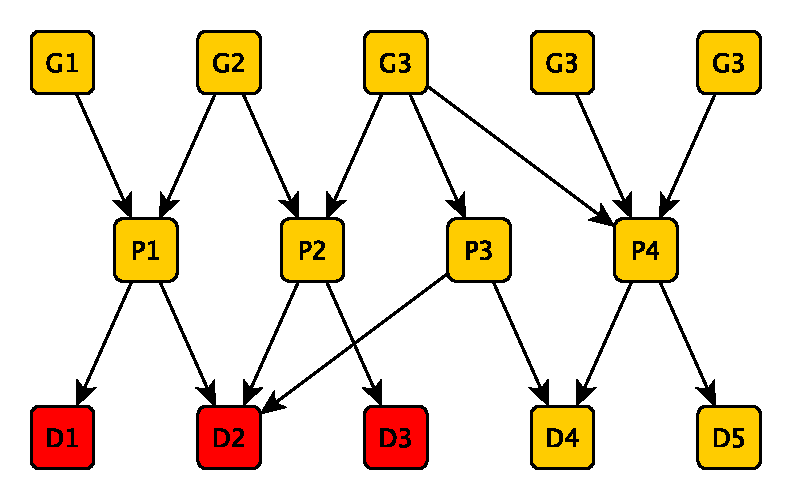
\includegraphics[scale=0.5]{img/network3-drivers.pdf}}

The drivers shown in red are impacted by the forked tuple from our starting point, \G2.

\section{Deriving co-generators}

Whereas a generator, such as \G2, produces a \textbf{fork}, that is a tuple addition or removal, there is a need to incorporate the values for other, related generators, the so-called co-generators.  The original generator produces a single value, for we will need to iterate over all values that have already been generated by co-generators, to be able to produce all the newly initiated output to send to drivers.  Well, after applying conditions, that is.

\subsection{Co-generators for complete production of \G2}

To provide the impacted drivers with input, we need to be able to produce variable values from a number of partitions, of course constrained by the conditions that apply to them.  The partititons that apply here contain at least the partitions discovered during the downward movement (shown in red) so we draw these upward addition of \P3 in green:

\centerline{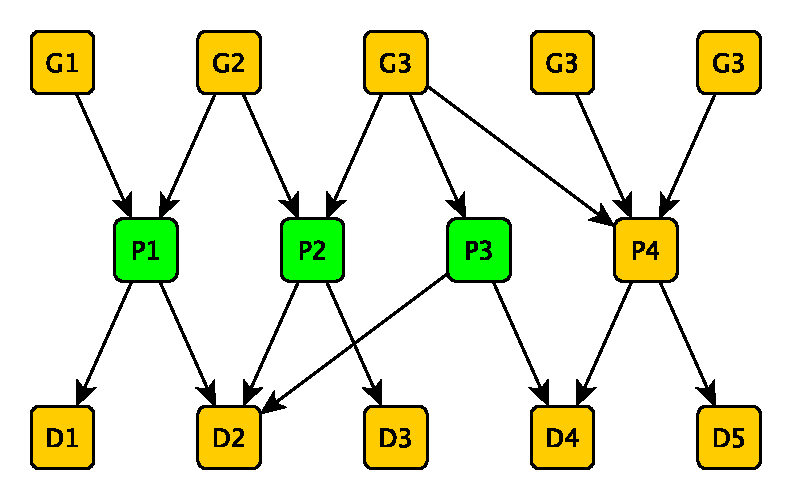
\includegraphics[scale=0.5]{img/network4-varsneeded.pdf}}

To be able to produce these variable partitions we need at least the original generator \G2, but there may be additional ones shown again in green; in this case, we also need \G1 and \G3:

\centerline{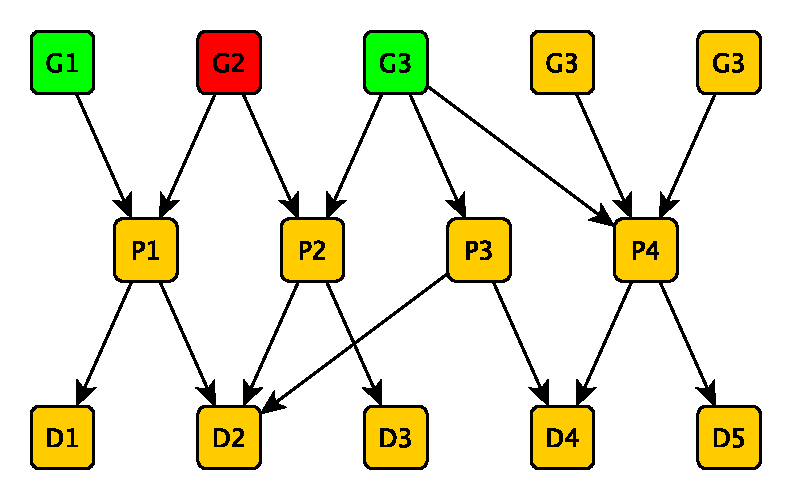
\includegraphics[scale=0.5]{img/network5-gensneeded.pdf}}

The additional generators in green, so \G1 and \G3, are called the \textbf{co-generators} needed for the production of the drivers impacted by our starting point, \G2 or, briefly put, they are the co-generators for the \textbf{complete production} of \G2.

Thanks to the two colours we can create an overview image, where green are the upward additions,

\centerline{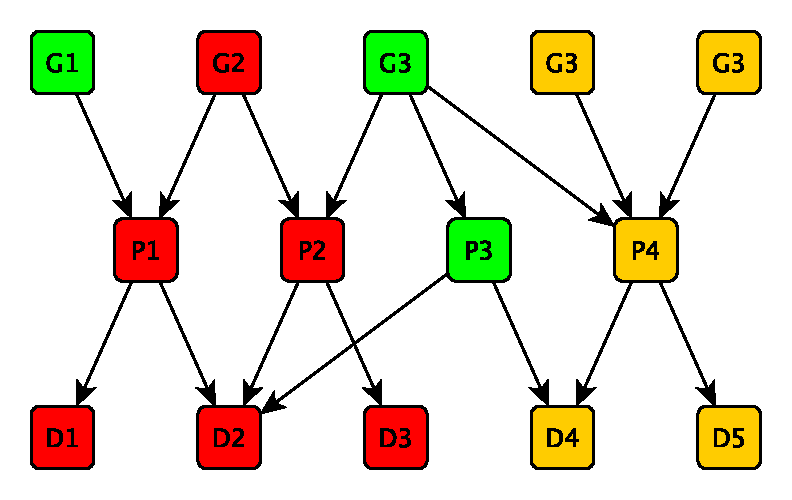
\includegraphics[scale=0.5]{img/network6-combined.pdf}}

\subsection{Co-generators of \G2 for production of \D1}

Implementations may vary in their ability to produce all impacted drivers at once; for our implementation on top of SQLite3 we produce only one driver at a time.  We will now look into the production of \D1 alone.

\centerline{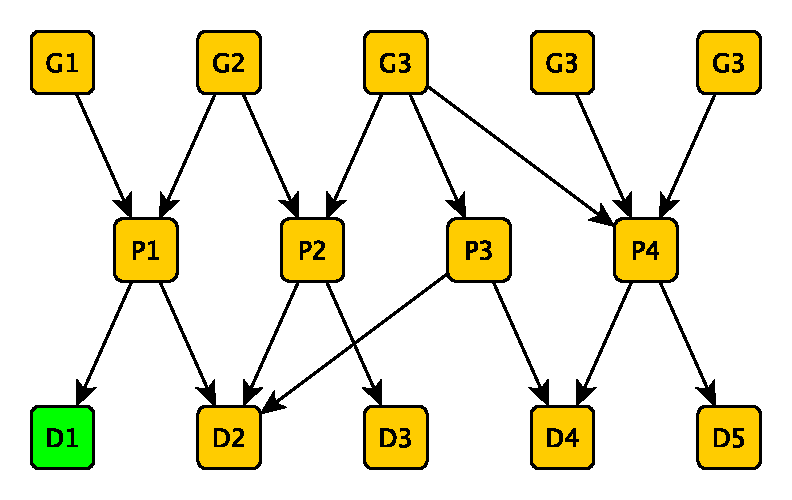
\includegraphics[scale=0.5]{img/network3-drivers-w1.pdf}}

This requires only \P1,

\centerline{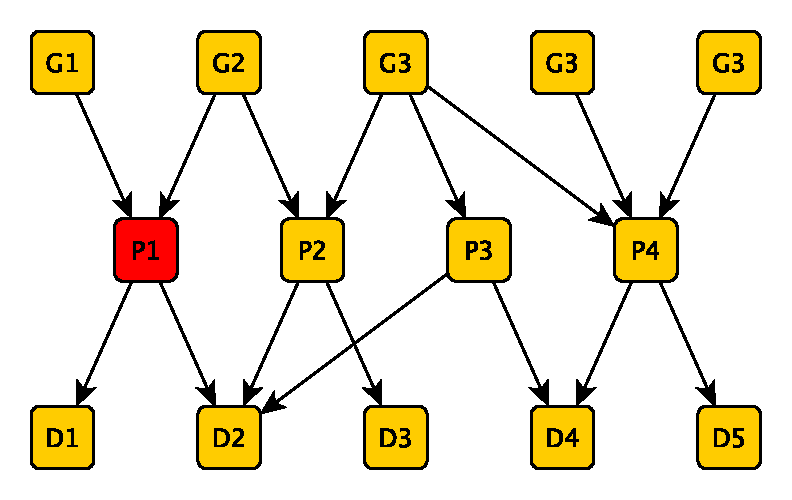
\includegraphics[scale=0.5]{img/network4-varsneeded-w1.pdf}}

For which we need to run \G1 and \G2,

\centerline{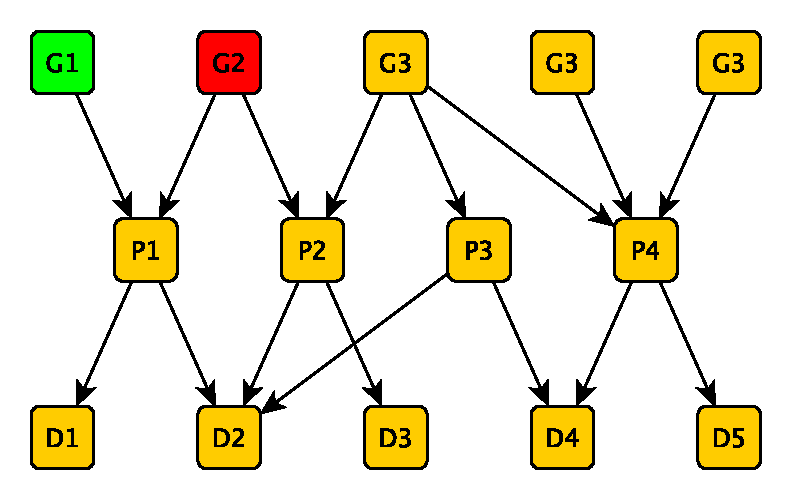
\includegraphics[scale=0.5]{img/network5-gensneeded-w1.pdf}}

In this case, \G1 is a co-generator to \G2 for the production of \D1.  This is much simpler than the general case.

\subsection{Co-generators of \G2 for production of \D2}

We now turn to another production, namely for output \D2.  As this will demonstrate, we may not always find simpler outcomes by looking at single drivers at a time.

\centerline{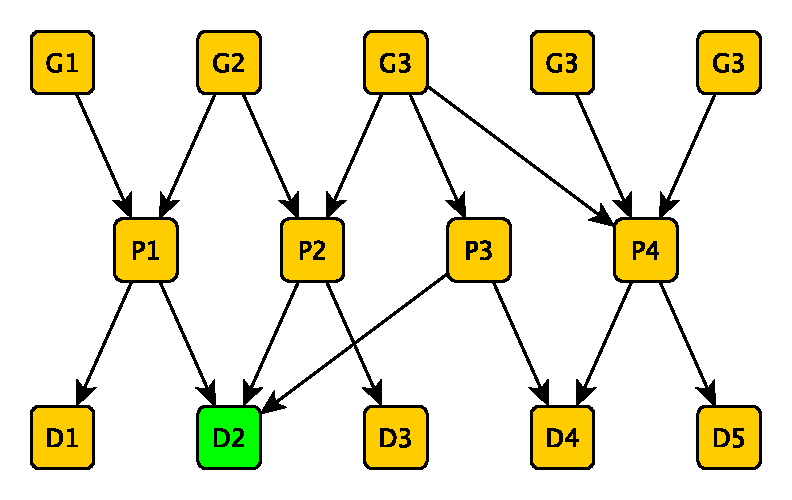
\includegraphics[scale=0.5]{img/network3-drivers-w2.pdf}}

This requires \P1, \P2 and \P3,

\centerline{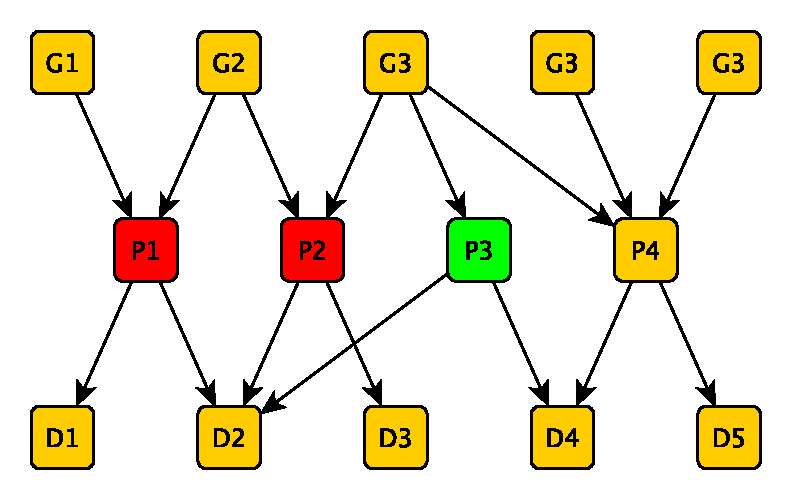
\includegraphics[scale=0.5]{img/network4-varsneeded-w2.pdf}}

For which we need to run \G1, \G2 and \G3, just as in the general case,

\centerline{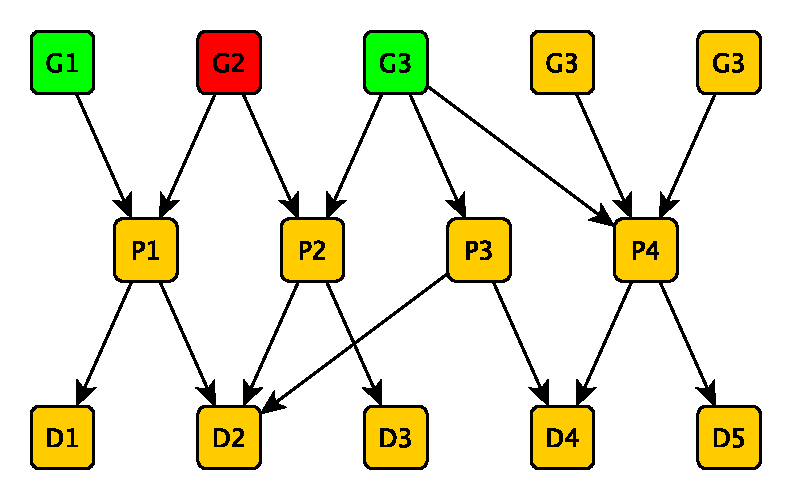
\includegraphics[scale=0.5]{img/network5-gensneeded-w2.pdf}}

In this case, \G1 and \G3 are the co-generators to \G2 for the production of \D2.

\section{Determining guards for drivers}

A driver outputs variables, but not necessarily the precise amount that is generated by a production from the Pulley script. Even when only the co-generators for its specific output are produced, then the variable partitions involved may still supply extra variables that are not passed on to the driver as output.

Variables that are produced alongside the variables for a driver's output are called \textbf{guards}.  When they are not explicitly declared by a user, they count as \textbf{implicit guards}.  They are important because productions create unique combinations of guards plus output, but output on its own may not be unique and require the guard as add-on information.  Drivers may take guards into account to make this possible, or the Pulley could count how many guards were produced for a given output.  To that end, it could store the output (or a hash of the output) together with a counter.

When co-generators are derived for the production of output for multiple drivers at once, then guards may be larger than when a generating them for a single driver.  The principle remains the same, although optimisations may exist.

\section{Producing output from a fork}

Given the addition or removal of a fork by a generator, we need to produce output, either adding or removing them through various. driver.  We first derive impacted drivers, and co-generators for either one driver are all at once; the following applies to both but require repeating when multiple drivers are separately considered.

\begin{enumerate}
\item Bind the forked tuple to its variables.
\item Run all co-generators in a nested fashion to produce their cartesian product.
\item Bind the elements of the cartesian product to their variables.
\item Skip further processing of variable bindings that fail on one of the conditions defined for the used variable partitions.
\item For each driver, hash the output values and increment its use count.
\item When the output values are new on addition, send an addition to the driver.
\item When the output values are removed for the last time, send a removal to the driver.
\end{enumerate}

This procedure ensures that output is generated by a driver for as long as at least one of its entries occurs in the LDAP system.  Some drivers may however accept the addition of guards, which makes them responsible of managing the multiplicity from these extra variables.  There is no reason why this could be problematic, as the guards will be as consistent on reproduction as are the normal output variables.

\section{Compiling the Pulley script language}

The compiler built into Pulley performs a fair amount of semantic analysis to be able to produce the incremental output for drivers.  The result of the analysis is a series of SQLite3 queries, aimed at producing one driver at a time (and running multiple of these as a result of a single generator fork).

\subsection{Storage model}
 
The SQLite3 database holds the following information:

\begin{itemize}
\item\textbf{Generator tuples}, holding each of the variable values as a separate blob.  These tables are extended when a fork is added, and reduced when a fork is removed.  They are used to produce the cartesian product when the generator serves as a co-generator.  Generators that never serve as co-generators do not need this table.
\item\textbf{Driver output use-counts}, stored as a hash over the output variables (in their normal order) together with the number of fork additions minus the number of fork removals.  When not in the table, the use-count is considered 0.  Transitions from 0 to 1 cause the driver to be supplied with an output addition, and transitions from 1 to 0 cause the driver to be supplied with an output removal.  This is not required when an output has no guards, or when it handles the guards internally.
\end{itemize}

\subsection{Global process of the Pulley script Compiler}

The following phases define the broad processing of the Pulley compiler:

\begin{enumerate}
\item\textbf{Download} of the Pulley script from LDAP and/or files into the re-entrant parser is possible, because it consists of lines without structure, and processing does not depend on the order of occurrence of the lines.
\item\textbf{Hashing} of individual lines, and their combination to an overall script hash in an order-independent manner support a quick check whether the Pulley script has changed.  This is instrumental for fast restarts; complete reset of the output is only required when the Pulley script changes and when SyncRepl updates over LDAP fails.
\item\textbf{Parsing} introduces new variables in generators, each time using a unique name.  Initially, each variable is assigned to a unique partition.
\item\textbf{Analysis} produces knowledge about variable partitions and co-generators, initially targeted at a single driver at a time.
\item\textbf{Production} produces the computation rules for an engine, initially SQLite3 with generation of queries that process generator forks and produce output through drivers.
\end{enumerate}

\subsection{Analysis of a Pulley script}

The analysis phase is the most complex phase during compilation, and is summarised by the images presented before.  The following steps are taken during the analysis phase:
\begin{enumerate}
\item\textbf{Structural analysis} derives variable partitions and the things a driver needs for its work, and the things a generator needs for its work.
\item\textbf{Structural consistency} validates that every variables is bound by precisely one generator, that every condition contains at least one variable and that driver output always contains at least one variable.
\item\textbf{Cost analysis} is not needed with the SQLite3 engine; it analyses the cheapest generators through estimated costs; this is overtaken by the analysis done by SQLite3 during query optimisation.
\item\textbf{Generate paths} is not needed with the SQLite3 engine; it produces what is thought to be the cheapest path, known as the \textbf{path of least resistence}, for production of output for drivers.
\end{enumerate}

\end{document}
